\documentclass[a4paper,12pt]{article}
\usepackage{tikz}
\usetikzlibrary{calc}
\usetikzlibrary{arrows}
\usetikzlibrary{automata}
\usetikzlibrary{backgrounds}
\usetikzlibrary{decorations}
\begin{document}
\pagestyle{empty}
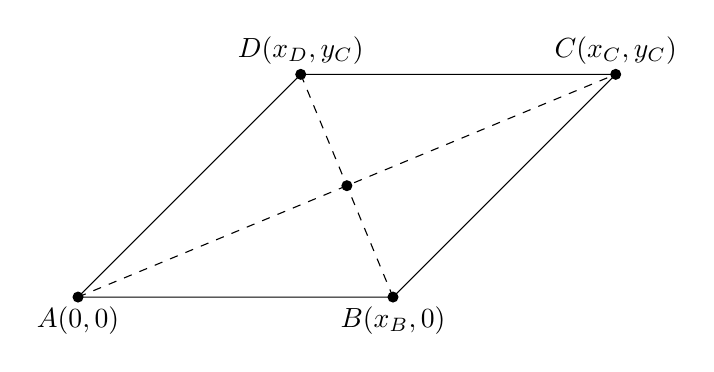
\begin{tikzpicture}[scale=1.0]
    \coordinate (A) at (0,0);
    \coordinate (B) at (4,0);
    \coordinate (D) at ($(A)!1!45:(B)$);
    \coordinate (C) at ($(D) + (4,0)$);

    \draw[solid] (A) -- (B) -- (C) -- (D) -- cycle;

    \draw[dashed] (A) -- (C);
    \draw[dashed] (B) -- (D);

    \coordinate (E) at (intersection of A--C and B--D) {};

    \node [below] at (A) {$A(0, 0)$};
    \node [below] at (B) {$B(x_B, 0)$};
    \node [above] at (C) {$C(x_C, y_C)$};
    \node [above] at (D) {$D(x_D, y_C)$};

    \fill[black] (A) circle (2pt);
    \fill[black] (B) circle (2pt);
    \fill[black] (C) circle (2pt);
    \fill[black] (D) circle (2pt);
    \fill[black] (E) circle (2pt);
\end{tikzpicture}
\end{document}

